\begin{frame}
  \frametitle{Economic geology (I)}

  One way that gold deposits form is by having Au chloride fluids rise
  from the deep earth, wash over cyanobacteria colonies, and reduce to
  metallic gold.

  \begin{columns}
    \begin{column}{0.5\linewidth}
      \includegraphics[width=\linewidth]{aucl/aucl_exp.pdf}
    \end{column}
    \begin{column}{0.5\linewidth}
      We simulated this process at the beamline by exposing
      cyanobacteria to an Au$^{3+}$ solution and ``watching'' the
      evolution of the Au XAS from Au$^{3+}$ to Au$^0$.
      \begin{block}{Questions}
        \begin{itemize}
        \item What is the rate constant?
        \item Is there an intermediate species?
        \end{itemize}
      \end{block}
    \end{column}
  \end{columns}

  \begin{textblock*}{0.5\linewidth}(0pt,18.5\TPVertModule) 
    \tiny
    M. Lengke et el., \textit{Mechanisms of Gold Bioaccumulation by
      Filamentous Cyanobacteria from Gold(III)-Chloride Complex},
    Environ. Sci. Technol. \textbf{40}(20) p.~6304-6309. (2006),
    \href{http://dx.doi.org/10.1021/es061040r}
    {\color{Blue4}\texttt{DOI: 10.1021/es061040r}}
  \end{textblock*}
\end{frame}
\begin{frame}
  \frametitle{Economic geology (II)}

  \begin{columns}
    \begin{column}{0.5\linewidth}
      We see that \alert{7 minutes} after injection, the data strongly
      resemble the {\color{Blue3}Au$^{3+}$Cl}.  After
      {\color{Purple4}one week}, the data resemble
      {\color{Green4}Au metal}.\\[1ex]
      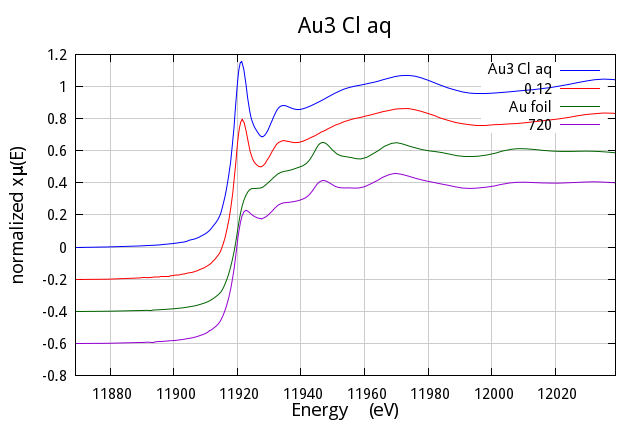
\includegraphics[width=\linewidth]{aucl/aucl_data.png}
    \end{column}
    \begin{column}{0.5\linewidth}
      Over the course of the time series, the white line $\sim11921$
      shrinks while the bump $\sim11945$ grows, suggesting the
      reduction to Au metal.\\[1ex]
      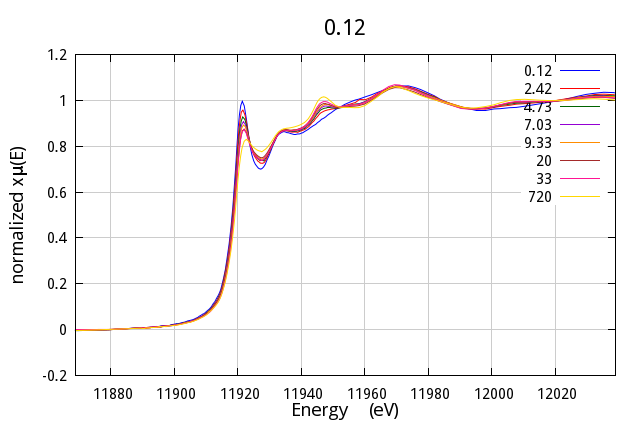
\includegraphics[width=\linewidth]{aucl/aucl_time.png}
    \end{column}
  \end{columns}

  \begin{textblock*}{0.5\linewidth}(0pt,18.5\TPVertModule) 
    \tiny
    M. Lengke et el., \textit{Mechanisms of Gold Bioaccumulation by
      Filamentous Cyanobacteria from Gold(III)-Chloride Complex},
    Environ. Sci. Technol. \textbf{40}(20) p.~6304-6309. (2006),
    \href{http://dx.doi.org/10.1021/es061040r}
    {\color{Blue4}\texttt{DOI: 10.1021/es061040r}}
  \end{textblock*}
\end{frame}
\begin{frame}
  \frametitle{Economic geology (III)}

  \begin{columns}
    \begin{column}{0.5\linewidth}
      We can analyze these data as a linear combination of species,
      including {\color{Green4}Au$^{3+}$Cl}, {\color{Purple4}Au
        metal}, and {\color{Orange2}Au$^{1+}$ sulfide}.\\[1ex]
      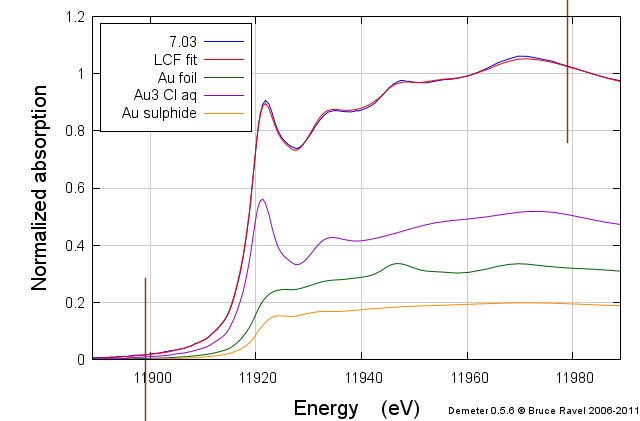
\includegraphics[width=\linewidth]{aucl/aucl_lcf.png}
    \end{column}
    \begin{column}{0.5\linewidth}
      We can plot out the contributions from these species as a
      function of time to get a sense of reaction rates.\\[1ex]
      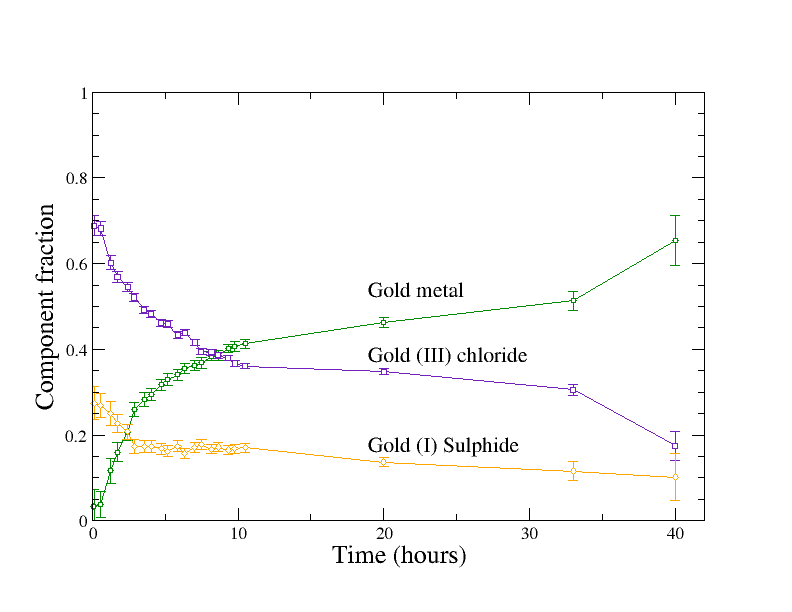
\includegraphics[width=\linewidth]{aucl/aucl_results.png}
    \end{column}
  \end{columns}

  \begin{textblock*}{0.5\linewidth}(0pt,18.5\TPVertModule) 
    \tiny
    M. Lengke et el., \textit{Mechanisms of Gold Bioaccumulation by
      Filamentous Cyanobacteria from Gold(III)-Chloride Complex},
    Environ. Sci. Technol. \textbf{40}(20) p.~6304-6309. (2006),
    \href{http://dx.doi.org/10.1021/es061040r}
    {\color{Blue4}\texttt{DOI: 10.1021/es061040r}}
  \end{textblock*}
\end{frame}
